\documentclass[tikz,border=8pt]{standalone}
\usepackage{amsmath,amssymb}
\usetikzlibrary{arrows.meta,calc,decorations.markings}

\begin{document}
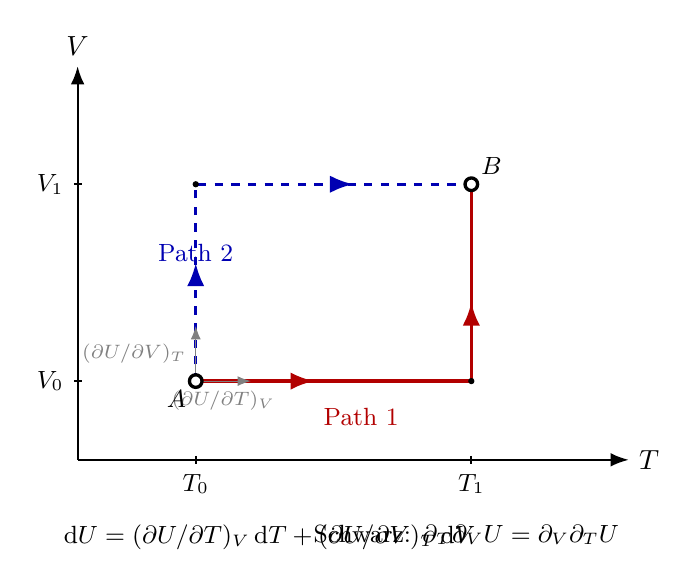
\begin{tikzpicture}[>=Latex,
  pathone/.style={very thick, red!70!black,
    postaction={decorate, decoration={markings,
      mark=at position 0.25 with {\arrow{>}},
      mark=at position 0.75 with {\arrow{>}}}}},
  pathtwo/.style={very thick, blue!70!black, dashed,
    postaction={decorate, decoration={markings,
      mark=at position 0.25 with {\arrow{>}},
      mark=at position 0.75 with {\arrow{>}}}}}]

  % axes
  \draw[->, thick] (0,0)--(7,0) node[right]{$T$};
  \draw[->, thick] (0,0)--(0,5) node[above]{$V$};

  \coordinate (A)  at (1.5, 1.0);
  \coordinate (B)  at (5.0, 3.5);
  \coordinate (C1) at (5.0, 1.0);
  \coordinate (C2) at (1.5, 3.5);

  % path 1 (A -> C1 -> B): along V0 then T1
  \draw[pathone] (A) -- (C1) -- (B);
  % path 2 (A -> C2 -> B): along T0 then V1
  \draw[pathtwo] (A) -- (C2) -- (B);

  % partial derivative arrows at A
  \draw[->, thin, gray] (A)--++(0.7, 0) node[midway, below, font=\scriptsize, gray]{$(\partial U/\partial T)_V$};
  \draw[->, thin, gray] (A)--++(0, 0.7) node[midway, left, font=\scriptsize, gray]{$(\partial U/\partial V)_T$};

  % point markers
  \draw[fill=white, very thick] (A) circle (0.08);
  \draw[fill=white, very thick] (B) circle (0.08);
  \fill[black] (C1) circle (0.04);
  \fill[black] (C2) circle (0.04);

  % axis ticks
  \draw[thick] (1.5,0.05)--(1.5,-0.05) node[below, font=\small]{$T_0$};
  \draw[thick] (5.0,0.05)--(5.0,-0.05) node[below, font=\small]{$T_1$};
  \draw[thick] (0.05,1.0)--(-0.05,1.0) node[left, font=\small]{$V_0$};
  \draw[thick] (0.05,3.5)--(-0.05,3.5) node[left, font=\small]{$V_1$};

  % point labels
  \node[below left, font=\small] at (A) {$A$};
  \node[above right, font=\small] at (B) {$B$};

  % path labels
  \node[red!70!black, font=\small, anchor=west] at (3.0, 0.55) {Path 1};
  \node[blue!70!black, font=\small, anchor=south] at (1.5, 2.4) {Path 2};

  % formulas (below)
  \node[align=left, font=\small, anchor=north west] at (-0.3, -0.7)
    {$\mathrm{d}U=(\partial U/\partial T)_V\,\mathrm{d}T+(\partial U/\partial V)_T\,\mathrm{d}V$};
  \node[align=right, font=\small, anchor=north east] at (7.0, -0.7)
    {Schwarz: $\partial_T\partial_V U=\partial_V\partial_T U$};
\end{tikzpicture}
\end{document}
